\documentclass{article}

\usepackage{tikz}
\usepackage{ifthen}
\usetikzlibrary{math}
\begin{document}
\pagestyle{empty}

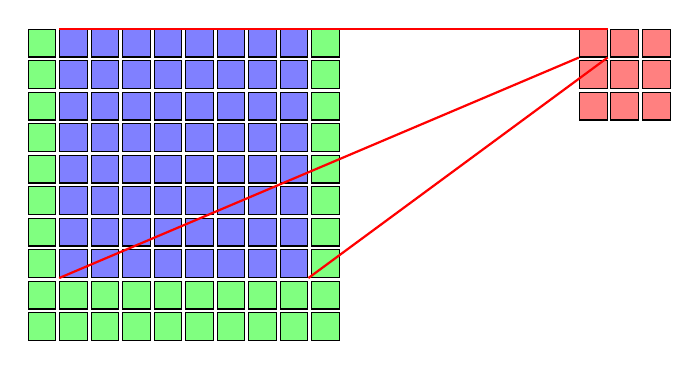
\begin{tikzpicture}[draw=black!50]
\tikzstyle{neuron}=[rectangle, draw=black, fill=black!25, minimum size=10pt]
\tikzstyle{input neuron}=[neuron, fill=green!50];
\tikzstyle{output neuron}=[neuron, fill=blue!50];
\tikzstyle{kernel neuron}=[neuron, fill=red!50];
\tikzstyle{annot} = [text width=4em, text centered]
\tikzstyle{kline} = [red, thick]

% Draw the input layer nodes
\tikzmath{
    \scalenn = 0.4;
    \inputsize = 10;
    \outputsize = 8;
    \kernelsize = 3;
    \xstart = 1;
    \ystart = 0;
    \xend = \xstart + \outputsize + 1;
    \yend = \ystart + \outputsize + 1;
    int \bxstart, \bystart, \bxend, \byend;
    \bxstart = \xstart + 1;
    \bystart = \ystart + 1;
    \bxend = \xend - 1;
    \byend = \yend - 1;
}

\foreach \x in {1,...,\inputsize}
    \foreach \y in {1,...,\inputsize}
        \ifthenelse {\x > \xstart \and \x < \xend
            \and \y > \ystart \and \y < \yend}
        {
            \node[output neuron] (I-\x-\y) at (\x * \scalenn, -\y * \scalenn) {};
        }
        {% else
            \node[input neuron] (I-\x-\y) at (\x * \scalenn, -\y * \scalenn) {};
        };

\foreach \x in {1,...,\kernelsize}
    \foreach \y in {1,...,\kernelsize}
        \node[kernel neuron, xshift=7cm] (K-\x-\y) at (\x * \scalenn, -\y * \scalenn) {};

\draw [kline] (I-\bxstart-\bystart.north west) -- (K-1-1.north west);
\draw [kline] (I-\bxend-\bystart.north east) -- (K-1-1.north east);
\draw [kline] (I-\bxstart-\byend.south west) -- (K-1-1.south west);
\draw [kline] (I-\bxend-\byend.south east) -- (K-1-1.south east);

\end{tikzpicture}
% End of code
\end{document}
